\section{Data}
\subsection{Vital Statistics Natality Data}
Our data on WIC births is taken from restricted-use Vital Statistics Natality Database. Natality data is coded from birth certificates, which includes birth and parental information such as county of maternal residence, year of birth, and mothers' age, educational attainment, marital status, and WIC participation, etc. The 2003 revision of birth certificate requires addition of mothers' WIC participation. But this information was not available until 2009. We collapse the birth-level natality data to
county-of-maternal-residence-by-year-of-birth cells to make the sample size more manageable. Our sample period spans 2009-2021.

Ideally, we would like to construct our sample with only mothers eligible for WIC. Since we do not observe WIC eligibility or maternal income from birth certificate, we focus on less-educated and unmarried (LEUM) mothers as they are more likely to be eligible for WIC. This is a common approach to study policy impacts when we cannot tell who is the target of policy \citep{meckel2020cure,alsan2022fear, east2023labor}. \cite{meckel2020cure} create a "high poverty" indicator taking into account whether mother is non-white Hispanic or black, whether mother is unmarried, and whether mother has a high school education or less as a proxy for maternal income. We choose LEUM status over this high poverty indicator because a nontrivial amount of counties in our sample have few births to qualified mothers, especially the minority (as in Figure \ref{proxy}). To still be able to capture lower-income mothers while removing minority as one of the criteria, we focus on those with more restrictive educational backgrounds: mothers with less than high school education. Indeed, WIC participation rate among LEUM mothers is 73.62\%, similar to the participation rate among \cite{meckel2020cure}'s sample (79.90\%), and much higher than the total participation among all mothers, which is 43.15\%. We test sensitivity of our results to alternative proxies.

\begin{figure}
	\begin{center}
		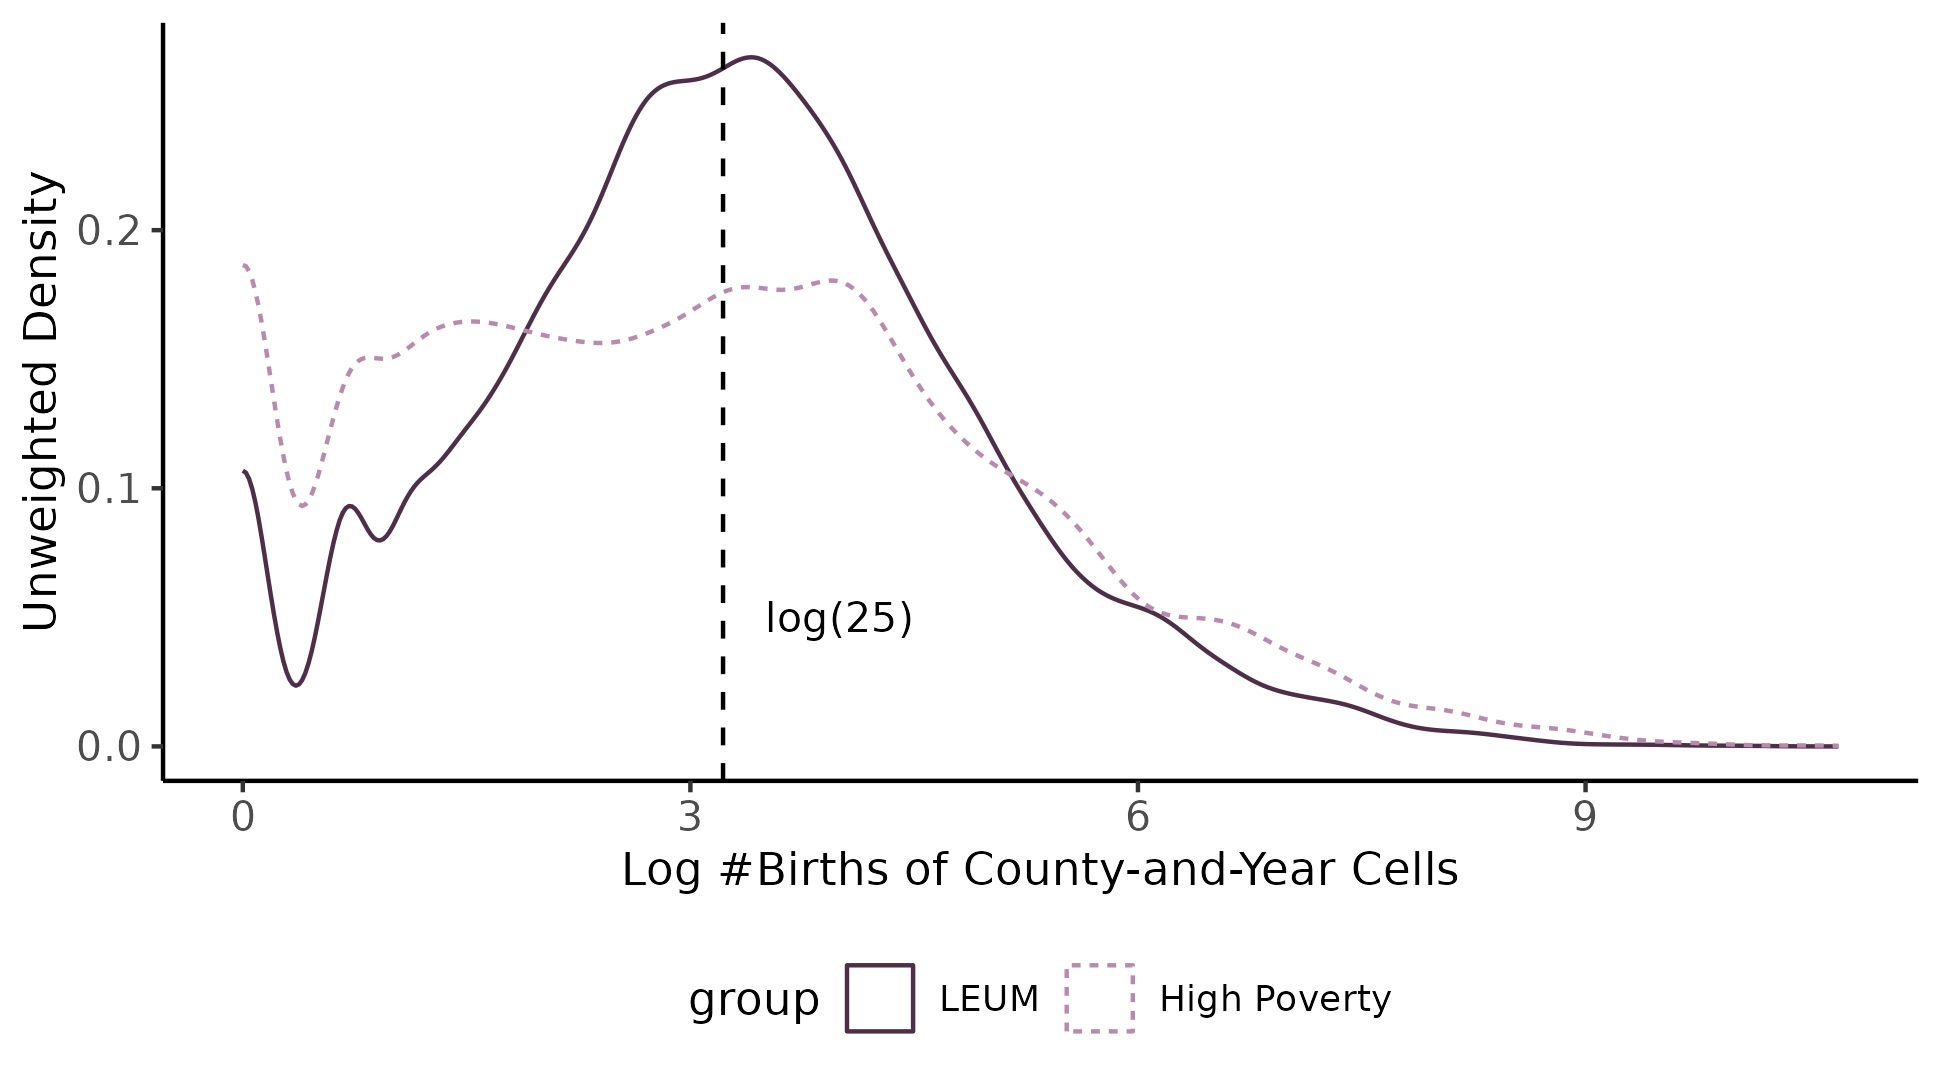
\includegraphics[width=.8\textwidth]{leum_hp.png}  
		\caption{\textsc{Comparing LEUM and High Poverty as Lower Limits for Cells}}
		\label{proxy}
	\end{center}
	\footnotesize
	Notes: The dashed line represents the distribution from the overlapped subset of \cite{meckel2020cure}'s data set. The solid line represents the distribution from the overlapped subset of our data set. They are almost identical.
\end{figure}

We validate our data by cross-checking whether the natality data from Vital Statistics are consistent with the birth data from Texas Department of State Health Services (Texas DSHS) used in \cite{meckel2020cure}. \cite{meckel2020cure}'s natality data from Texas DSHS covers births in counties implementing WIC EBT before April 2009 (239 counties) from January 2005 to December 2009. Our natality data covers births in all counties in Texas (254 counties) but only traces back to January 2009. Therefore, the overlapped subsets of two data sets cover births in counties implementing WIC EBT before April 2009, from January 2009 to December 2009. We compare the overlapped subsets of two data sets and find they are almost identical (as in Figure \ref{check}). 

\begin{figure}
	\begin{center}
		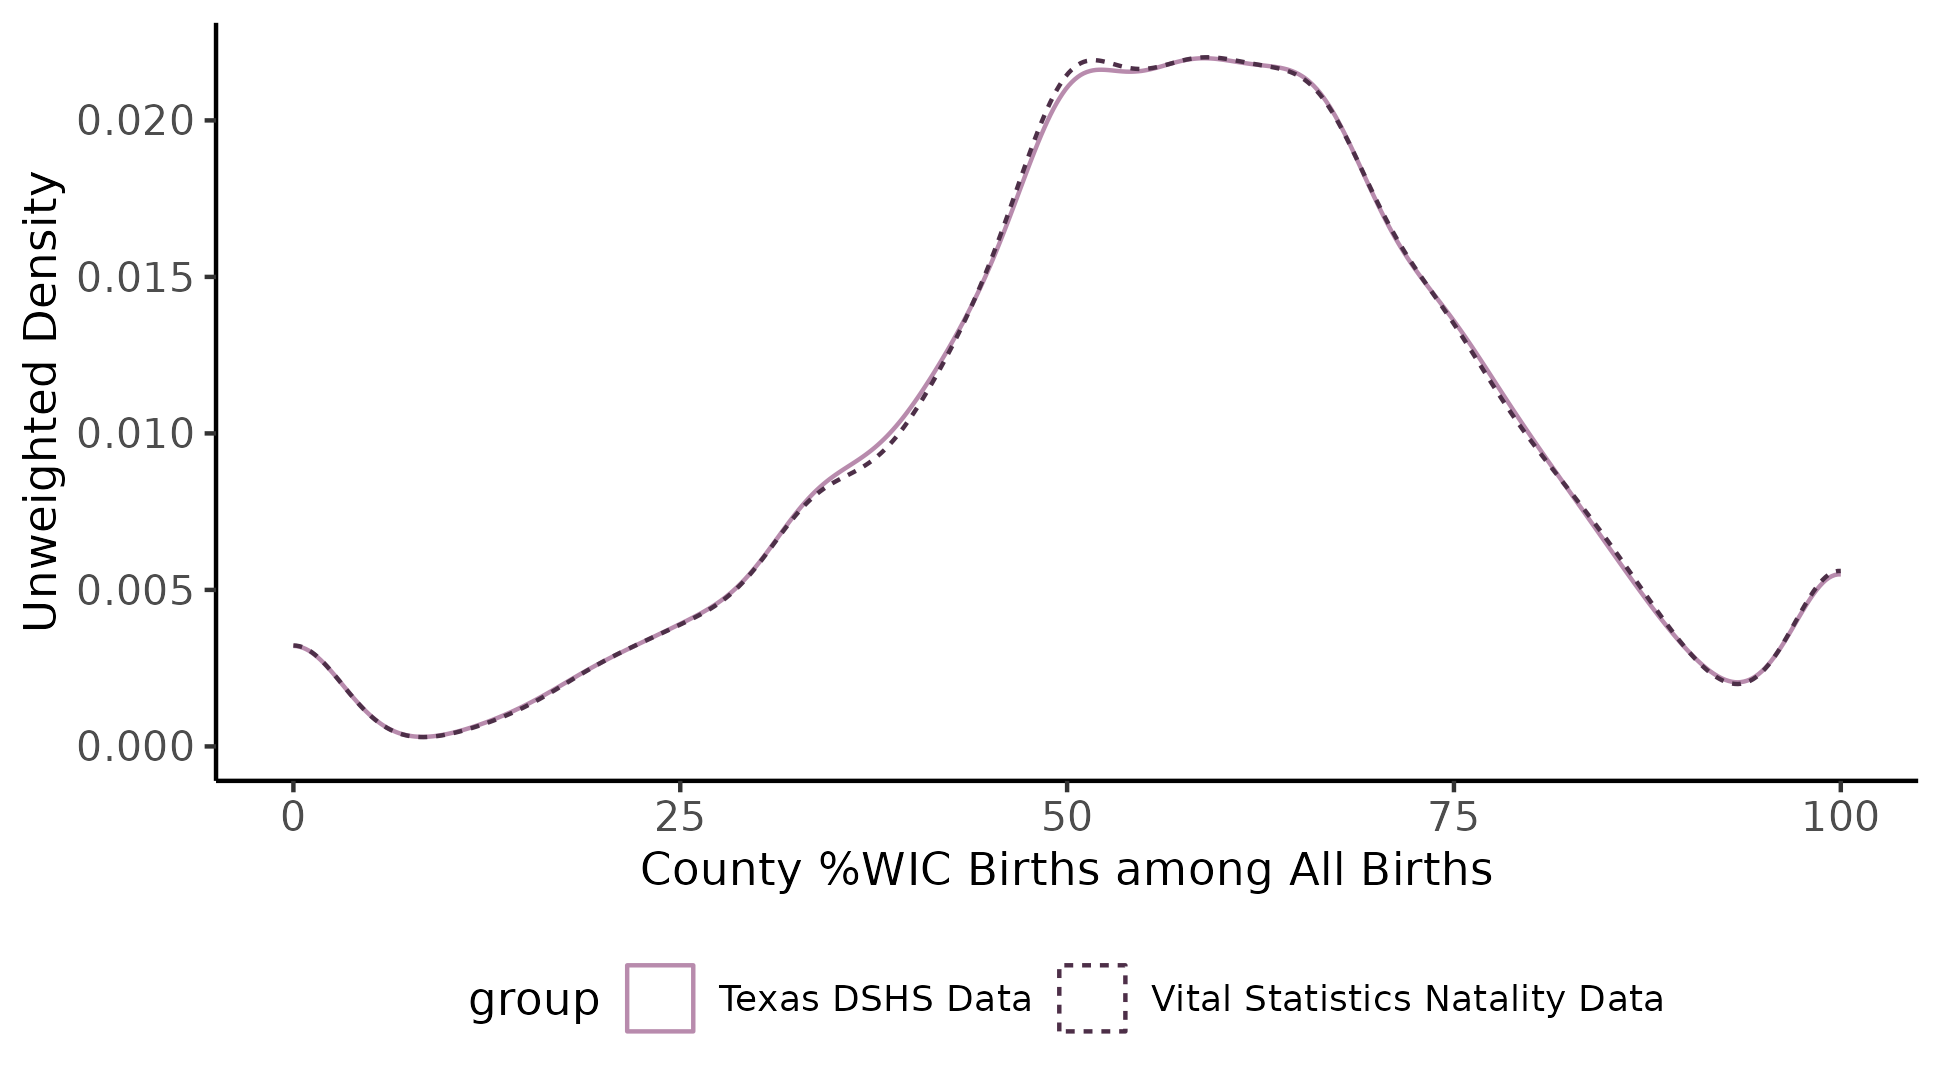
\includegraphics[width=.8\textwidth]{density_wic_rate.png}  
		\caption{\textsc{Distribution of County-level Share of WIC Birth}}
		\label{check}
	\end{center}
	\footnotesize
\end{figure}

\subsection{WIC EBT Roll-out}
We compile the WIC EBT rollout schedule across virtually all counties\footnote{Indian Tribal Organizations with separate WIC EBT implementation plans are excluded.} in the U.S. from public record of state WIC agencies. For counties reporting a range of implementation dates, we use the start date of that range. The county-level WIC EBT rollout is in Figure \ref{map}. We observation both cross- and within-state variation in timing of WIC implementation with cross-state variation dominating. Further excluding counties without reporting WIC participation, we end up a sample covering 2,549 counties, accounting for in total 81.24\% of population and 79.10 \% of births. Table \ref{included} presents baseline characteristics \footnote{These county baseline characteristics are chosen as they are likely to be correlated with the timing of WIC EBT implementation.} of our sample counties compared to those excluded counties. Included counties are not in general better off than excluded ones. Although included counties have smaller share of disadvantaged population, smaller share of infants with low birth weight, and receive more income maintenance benefits per person, they receive less SNAP benefit and have lower income per person. We do not observe significant difference in population size, per person reception of public assistance medical benefits, and net increase in WIC vendors between included and excluded counties. Table \ref{ebt_det} indicates that, while some county baseline characteristics are strongly correlated with the timing of WIC EBT implementation, they as a whole only explain a small share of the variation in implementation timing. Most of the variation in the timing of WIC EBT implementation is explained by state-level unobservables as R$^2$ becomes very close to 1 when state fixed effect is added. Therefore, the timing of the WIC EBT rollout can be considered plausibly exogenous after controlling for the county baseline characteristics.

\begin{figure}
	\begin{center}
		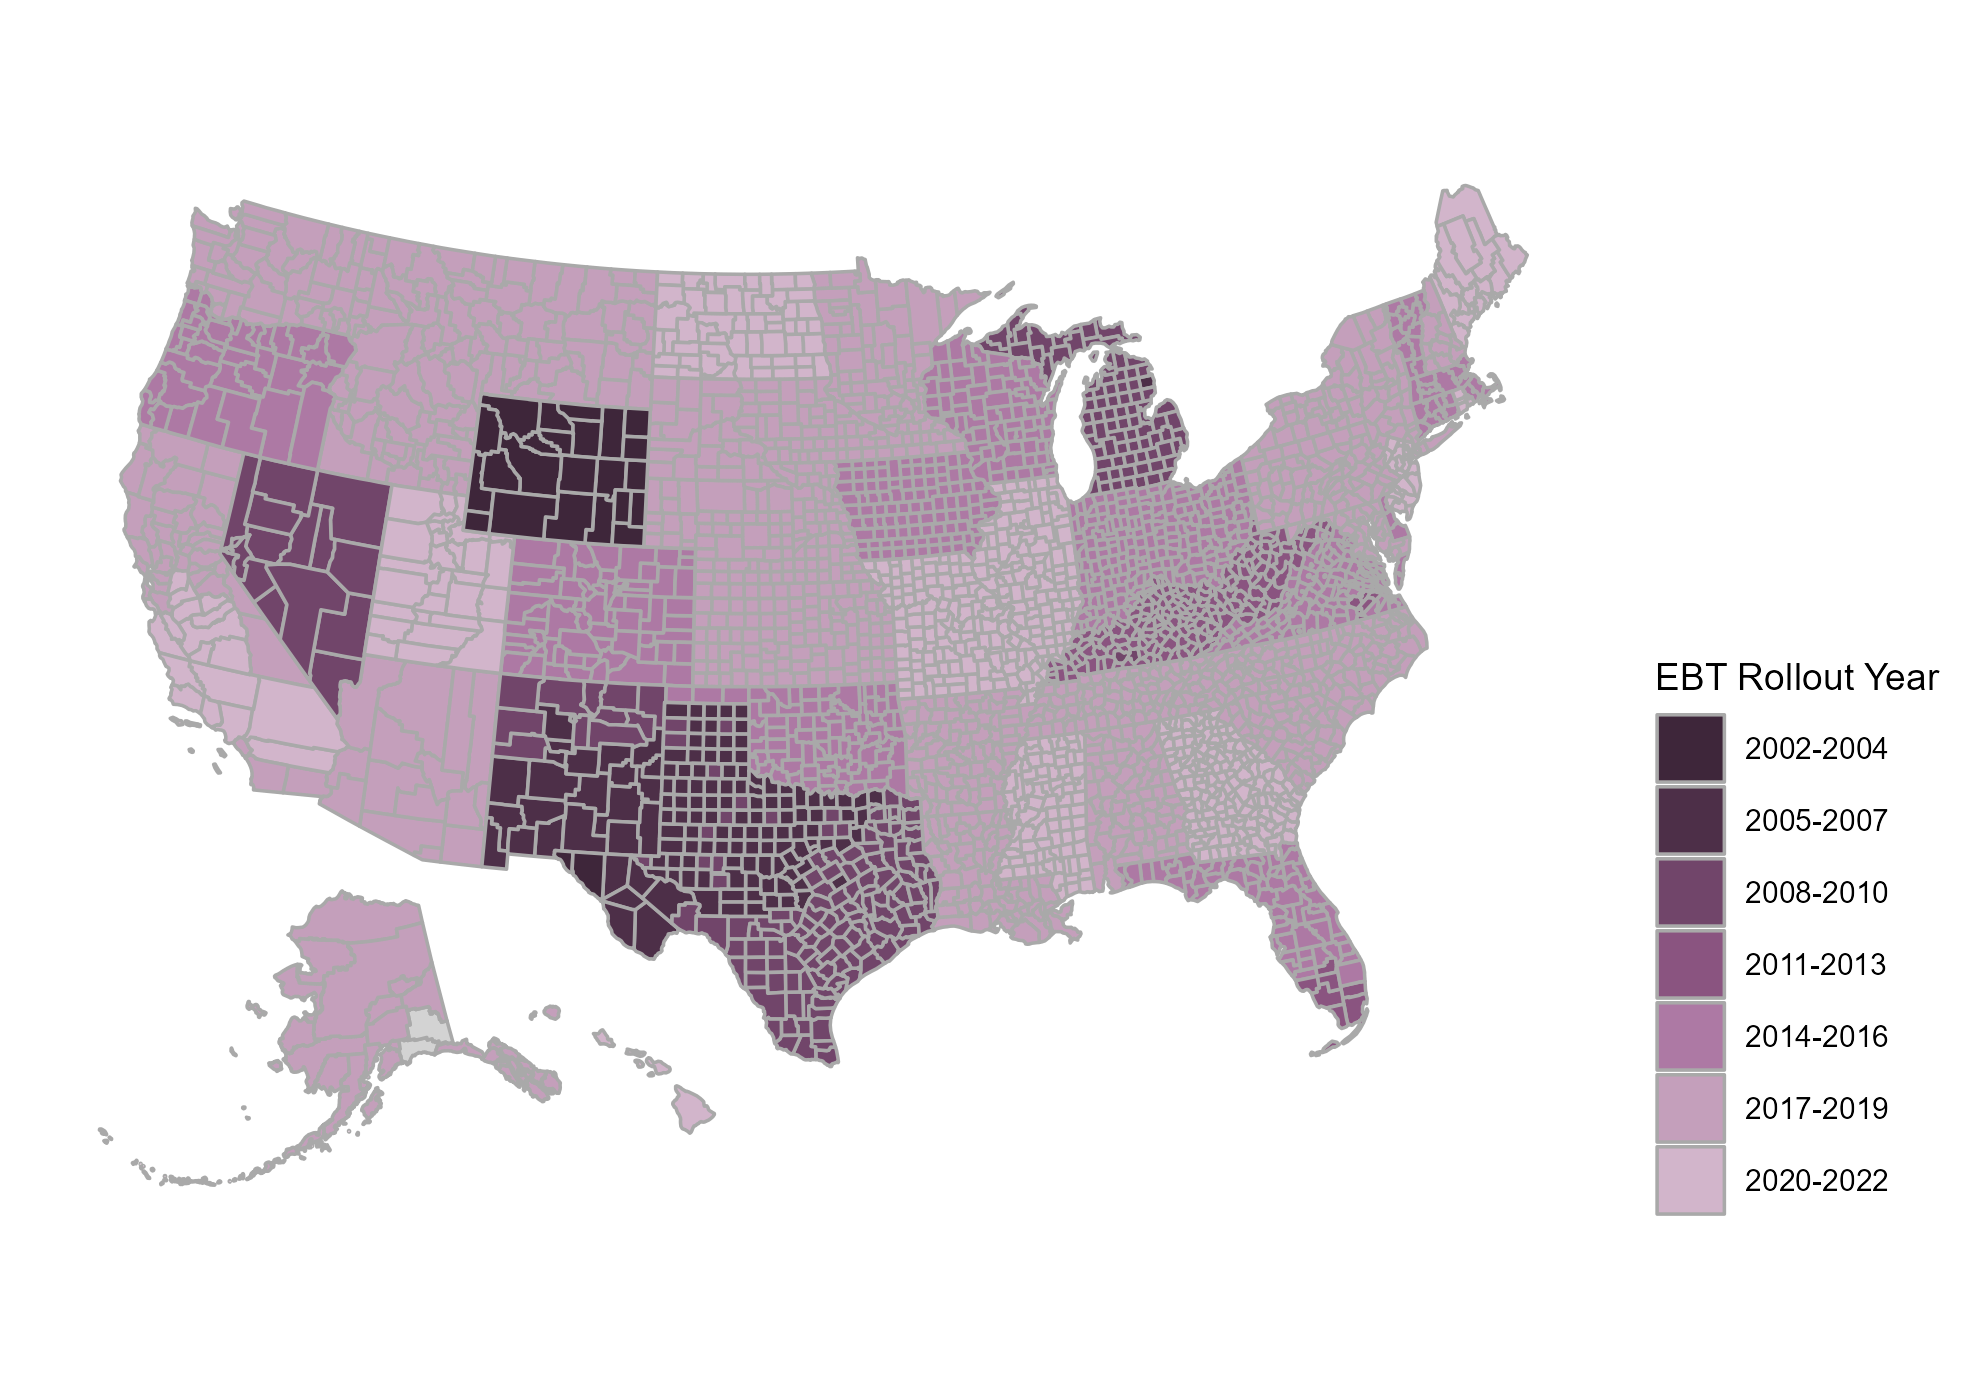
\includegraphics[width=.8\textwidth]{ewic_rollout_county_year.png}  
		\caption{\textsc{WIC EBT Roll-out Schedule}}
		\label{map}
	\end{center}
	\footnotesize
\end{figure}


\begin{table}[!htbp] 
	\begin{center}
		\caption{\textsc{Baseline Characteristics of Counties Included and Excluded in Sample}} 
		\label{included} 
		\footnotesize 
		\begin{tabular}{@{\extracolsep{0pt}}lccc } 
			\\[-1.8ex]\hline 
			\hline 
			\\[-1.8ex] & \multicolumn{1}{c}{Included} & \multicolumn{1}{c}{Excluded}& \multicolumn{1}{c}{Mean}\\ 
			\\[-1.8ex] & \multicolumn{1}{c}{Counties} & \multicolumn{1}{c}{Counties}& \multicolumn{1}{c}{Difference}\\ 
			\\[-1.8ex] & \multicolumn{1}{c}{(1)} & \multicolumn{1}{c}{(2)}& \multicolumn{1}{c}{(1) - (2)}\\ 
			\hline \\[-1.8ex] 
			\multicolumn{3}{l}{\textit{Demographics, 2006-2009}} & \\ 
			[1.2ex]
			\hspace{12pt} \% Black & 8.7877 & 11.8582 & -3.0705$^{***}$ \\ 
			& (0.2578) & (0.5407) & \\ 
			[1.2ex]
			\hspace{12pt} \% Hispanic &  5.4517 & 19.6239 & -14.1722$^{***}$ \\ 
			& (0.1464) & (0.8519) & \\ 
			[1.2ex]
			\hspace{12pt} \% Poor $\times$ Under Age 5 & 1.6745 & 1.9889 & -0.3143$^{***}$ \\ 
			& (0.0155) & (0.0344) & \\
			[1.2ex]
			\hspace{12pt} \% Low Birth Weight & 8.0111 & 8.7697 & -0.7587$^{***}$ \\ 
			& (0.0466) & (0.0972) & \\ 
			[1.2ex]
			\hspace{12pt} Population & 96,781 & 94,526 & 2,255\\ 
			& (6,302) & (11,228) & \\ 
			[1.2ex]
			\multicolumn{3}{l}{\textit{Transfers and Income, 2006-2009}} & \\ 
			[1.2ex]
			\hspace{12pt} Public Asst. Medical Benefits p.p. & 1.1536 & 1.1878 & -0.0341 \\
			\hspace{24pt} (incl., Medicaid)  & (0.0115) & (0.0220) & \\  
			[1.2ex]
			\hspace{12pt} Income Maintenance Benefits p.p. & 0.1961 & 0.1834 & 0.0127$^{***}$ \\ 
			\hspace{24pt} (incl., TANF and WIC Benefits)   & (0.0017) & (0.0028) & \\  
			[1.2ex]
			\hspace{12pt} SNAP Benefits p.p. & 0.1337 & 0.1472 & -0.0135$^{***}$ \\ 
			& (0.0017) & (0.0030) & \\ 
			[1.2ex]
			\hspace{12pt} Income p.p. (million) & 1.9681 & 2.0980 & -0.1299$^{***}$ \\ 
			& (0.0043) & (0.0098) & \\
			[1.2ex]
			\multicolumn{3}{l}{\textit{WIC Vendors, 2006-2009}} & \\ 
			[1.2ex]
			\hspace{12pt} Net Increase in WIC Vendors & 0.0508 & 0.0453 & 0.0055 \\ 
			\hspace{24pt} (thousand) & (0.0033) & (0.0050) & \\
			& &  &\\
			Number of Counties & 2,549 & 589 & \\ 
			Fraction of the Population & 81.24 & 18.76 &\\ 
			Fraction of Births & 	79.10 & 20.08 & \\ 
			\hline \\[-1.8ex] 
			\hline 
			\hline \\  [-5.0ex] 
		\end{tabular} 
	\end{center}
	\footnotesize
	Notes: (1) Fractions of the population and births do not sum up to 1 because we take into account observations without geographical identifiers. (2) Low birth weight is when birth weight is no more than 2,500 grams.
\end{table} 


\begin{table}[!htbp]
	\begin{center}
		\caption{\textsc{Determinants of WIC EBT Implementation Year}} 
		\label{ebt_det} 
		\footnotesize 
		\begin{tabular}{@{\extracolsep{0pt}}lcc } 
			\\[-1.8ex]\hline 
			\hline \\[-1.8ex] 
			& \multicolumn{2}{c}{\textit{Dependent variable:}} \\ 
			\cline{2-3} 
			\\[-1.8ex] & \multicolumn{2}{c}{Year of WIC EBT} \\
			\\[-1.8ex] & \multicolumn{2}{c}{Implementation, 2010-2021} \\
			\\[-1.8ex] & \multicolumn{1}{c}{(1)} & \multicolumn{1}{c}{(2)}\\ 
			\hline \\[-1.8ex] 
			\multicolumn{3}{l}{\textit{Demographics, 2006-2009}} \\ 
			[1.2ex]
			\hspace{12pt} \% Black & 0.0376$^{***}$ & -0.0020 \\ 
			 & (0.0116)   & (0.0020)\\   
			[1.2ex]
			\hspace{12pt} \% Hispanic &  0.0291$^{**}$ & 0.0121$^{***}$ \\ 
			& (0.0138)        & (0.0033)\\  
			[1.2ex]
			\hspace{12pt} \% Poor $\times$ Under Age 5 & -0.5638$^{*}$ & -0.1142$^{**}$ \\ 
			& (0.3002)        & (0.0444)\\ 
			[1.2ex]
			\hspace{12pt} \% Low Birth Weight & -0.3353$^{***}$ & -0.0140 \\ 
			& (0.0829)        & (0.0136)\\ 
			[1.2ex]
			\hspace{12pt} Log Population & -0.0895$^{**}$ & -0.0290$^{**}$ \\ 
			& (0.1026)        & (0.0129)\\
			[1.2ex]
			\multicolumn{3}{l}{\textit{Transfers and Income, 2006-2009}} \\ 
			[1.2ex]
			\hspace{12pt} Public Asst. Medical Benefits p.p. & 0.7369$^{***}$ & -0.0075 \\
			\hspace{24pt} (incl., Medicaid)  & (0.2474)        & (0.0444)\\  
			[1.2ex]
			\hspace{12pt} Income Maintenance Benefits p.p. & -3.7524$^{**}$ & 0.3763 \\ 
			\hspace{24pt} (incl., TANF and WIC Benefits)  & (1.708)     & (0.3672)\\  
			[1.2ex]
			\hspace{12pt} SNAP Benefits p.p. & 4.5554 & 1.2110$^{**}$ \\ 
			& (3.146)      & (0.4826)\\ 
			[1.2ex]
			\hspace{12pt} Income p.p. (million) & 2.1981$^{***}$ & 0.1769$^{**}$ \\ 
			& (0.4894)        & (0.0796)\\
			[1.2ex]
			\multicolumn{3}{l}{\textit{WIC Vendors, 2006-2009}} \\ 
			[1.2ex]
			\hspace{12pt} Net Increase in WIC Vendors & 0.3779$^{*}$ & 0.1081$^{***}$ \\ 
			
			\hspace{24pt} (thousand)  & (0.2154)        & (0.0361)\\   
			& & \\ 
			State Fixed Effects &  & \checkmark \\ 
			Observations & 2,549 & 2,549 \\ 
			R-squared & 0.1761 & 0.9893 \\ 
			\hline \\[-1.8ex] 
			\hline 
			\hline \\ [-5.0ex] 
		\end{tabular} 
	\end{center}
	\footnotesize
	Notes: (1) $^{***}$, $^{**}$, and $^{*}$ indicate that the estimates are significant at the 1\%, 5\%, and 10\% levels. (2) Each regression is weighted by the mean population during 2006-2009. (3) In parentheses are heteroscedasticity-robust standard error.
\end{table}


\subsection{County Baseline Characteristics}
We collect above county baseline characteristics from 2006-2009 from multiple sources. Our data on share of black, share of Hispanic, and income per person are from the American Community Survey (ACS) Public Use Microdata Sample. We construct our county-level ACS data by aggregating individual data with disclosed information on Public Use Microdata Areas (PUMA) to county level, weighted by ACS personal weight. We do not include observations from PUMA with population fewer than 100,000 since their geographic identifiers are suppressed. We cannot find county-level data for the same period on welfare programs that make participants automatically qualified for WIC except for SNAP. Instead, we collect county-level data on transfers that include these welfare programs from the Bureau of Economic Analysis, Regional Economic Information System (REIS). Public assistance medical benefits include benefits from Medicaid and other medical vendor payments. Income maintenance benefits consist largely of benefits from TANF, expenditures for food under WIC, and other general assistance such as tax credits, refugee assistance, foster home care and adoption assistance, and energy assistance. We also include county-level data on share of poor and under age 5 are from the Small Area Income and Poverty Estimates (SAIPE) Program, share of low birth weight from restricted-use Vital Statistics Natality Data, and net increase in WIC vendors from the WIC Integrity Profiles (TIP).

\section{Research Design}
To estimate the impact of WIC EBT on WIC participation, we compare shares of WIC births in counties that implemented WIC EBT with counties that have not yet implemented WIC EBT. We use a staggered difference-in-difference estimator from \cite{callaway2021difference} (hereafter CS estimator), which rules out the troubling issues due to negative weights in the two-way-fixed-effect estimator (TWFE estimator). The average treatment on the treated (ATT) of WIC EBT for the counties that were first treated in time $g$ at period $t$ conditional on covariates $X$ when using not-yet-treated groups as the comparison is:
\begin{align*}
	ATT (g, t; X) = & E[ Y_t - Y_{g-1} | X, G_g = 1 ] - E[Y_t - Y_{g-1} | X, G_g =0, D_t = 0],
\end{align*}
where $Y_t$ and $Y_{g-1}$ denote the potential outcome of the county-month-and-year cell in time $t$ and $g-1$, respectively, $G_g$ is a binary variable that is equal to one if a county is first treated in period $g$ and zero otherwise, $D_t$ is a binary variable that is equal to one if a county is treated in period $t$ and zero otherwise. $ATT(g, t; X)$ serves as the building blocks for a few estimates we are interested in. Our preferred estimate is the group-average overall ATT:
\begin{align*}
	ATT^{overall} & =\sum_g \sum_t  \frac{1}{T-g+1} \boldsymbol{1} \{ g \leq t \} P(G=g|G \leq t) ATT(g, t; X).
\end{align*}
$T$ is the time limit of the data set. To test pre-trend, we aggregate $ATT(g, t; X)$ using sample weights to get the dynamic effect in $l$ periods relative to event time $g$, denoted by $ATT^{dynamic}_{l}$ where $l = t - g$:
\begin{align*}
	ATT^{dynamic}_{l} & =  \sum_g  \boldsymbol{1}\{g + l \leq T\} P(G = g | G + l \leq T)ATT(g, g +l; X).
\end{align*}
CS estimator requires absorbing treatment. We do not realize any county in our sample that has abandoned EBT after initial implementation. Nevada redesigned and relaunched EBT in 2009 after implementing EBT earlier. But Nevada will not be included in our sample anyway since we need to drop all always treated counties including those implementing EBT in 2009. We then show our results still hold when using alternative staggered DD estimators.

We also report results from the following baseline TWFE estimator with county fixed effect and year fixed effect and use Goodman-bacon decomposition to examine its potential bias \citep{goodman2021difference}:
\begin{align*}
	Y_{ct} = \alpha + \mu EBT_{ct} + \lambda_t + \eta_c + \varepsilon_{ct},
\end{align*}
where $Y_{ct}$ is share of WIC Birth in county $c$ in year $t$, $\mu$ is the TWFE estimator of the impact of WIC EBT, $\lambda_t$ is year fixed effect, $\eta_c$ is county fixed effect, and $\varepsilon_{ct}$ is an error term.

Following prior work studying birth outcomes \citep{almond2011inside,hoynes2011can}, we drop all county-year cells with fewer than 25 births to avoid estimation problems associated with data thinness. Our results are robust to alternative lower limits for sample selection. All estimates are weighted using the number of births of cells and standard errors are clustered at county level.


